\chapter{Il reforming}
Con reforming intendiamo tutta quella serie di processi atti a migliorare le caratteristiche dei prodotti petroliferi tramite modificazione della struttura dei composti, in particolare si parte da benzine di prima distillazione (costituite da nafteni, cicloesani e paraffine lineari) per arrivare a benzine con N.O.\footnote{Ricordiamo che con il termine N.O. indichiamo il numero di ottano della benzina.} maggiori.
Altri prodotti desiderati sono strutture aromatiche, precursici di molti prodotti dell'industria petrolchimica, e idrogeno.

L'intero processo si basa su reazioni che trasformano paraffine lineari e nafteni in paraffine ramificate e aromatici (per esempio da cicloesano a benzene o \textit{n}-ottano in 2,2,3-trimetilpentano). Le reazioni principali che avvengono sono le \textit{deidrogenazioni ad aromatici}, l'\textit{isomerizzazione di paraffine lineari}, \textit{hydrocracking di paraffine} e le \textit{deidrociclizzazione di paraffine}.

Inizialmente (anni '30 e '40) il processo veniva compiuto per via termica, ovvero si operava a temperature di circa $580^oC$ e inserendo la carica questa veniva modificata senza necessitare di nessun catalizzatore; ci�, per�, portava a notevoli perdite di materia a causa di deidrogenazioni e reazioni indesiderate, per di pi� non consentiva di raggiungere N.O. superiori a 80. Per questi motivi attualmente si utilizza esclusivamente il reforming catalitico.

\section{Il reforming catalitico}
Come indicato precedentemente lo scopo del reforming catalitico � quello di migliorare le prestazioni delle benzine limitando le perdite dei reagenti iniziali e limitando le condizioni operative.

\subsection{Le reazioni}
Poich� il processo di reforming coinvolge una serie vasta di reazioni queste sono state raggruppate in alcune classi significative che ora andremo ad analizzare singolarmente.
\subsubsection{Deidrogenazioni}
Le deidrogenazioni sono reazioni endotermiche che quindi necessitano calore per avvenire, come evidente dal diagramma di Francis sono favorite dalle alte temperature ed in particolare possono essere considerate deidrogenazioni di alcani per dare alcheni:
\begin{equation}
	\vcenter{\hbox{\heptamethylene{}{}}}
	\rightarrow
	\vcenter{\hbox{\heptamethylene[e]{}{}}} + H_2
\end{equation}
da cicloalcani per dare aromatici:
\begin{equation}
	\vcenter{\hbox{\cyclohexanev{}{}}}
	\rightarrow
	\vcenter{\hbox{\cyclohexanev[A]{}{}}} + 3 H_2
\end{equation}
da cicloalcheni per dare aromatici:
\begin{equation}
	\vcenter{\hbox{\cyclohexanev[a]{}{}}}
	\rightarrow
	\vcenter{\hbox{\cyclohexanev[A]{}{}}} + 2 H_2
\end{equation}

\subsubsection{Deidroisomerizzazioni}
I questo caso un anello a paraffinico modifica la sua struttura e viene deidrogenato per dare un prodotto aromatico:
\begin{equation}
	\vcenter{\hbox{\fiveheterovi{}{1==$CH_3$}}}
	\rightarrow
	\vcenter{\hbox{\cyclohexanev{}{}}}
	\rightarrow
	\vcenter{\hbox{\cyclohexanev[A]{}{}}} + 3 H_2
\end{equation}

\subsubsection{Deidrociclizzazioni}
In questo caso una paraffina lineare subisce ciclizzazione per poi subire una aromatizzazione
\begin{equation}
	\vcenter{\hbox{\heptamethylene{}{}}}
	\rightarrow
	\vcenter{\hbox{\sixheterov{}{1==$CH_3$}}} + H_2
	\rightarrow
	\vcenter{\hbox{\sixheterov[A]{}{1==$CH_3$}}} + 4 H_2
\end{equation}
oppure si pu� partire da una olefina per avere chiusura ad anello e successiva aromatizzazione
\begin{equation}
	\vcenter{\hbox{\heptamethylene[d]{}{}}}
	\rightarrow
	\vcenter{\hbox{\sixheterov{}{1==$CH_3$}}}
	\rightarrow
	\vcenter{\hbox{\sixheterov[A]{}{1==$CH_3$}}} + 4 H_2
\end{equation}

\subsubsection{Isomerizzazioni}
Le isomerizzazioni portano a trasposizioni di alcuni gruppi per dare paraffine, olefine o aromatici con struttura modificata, per esempio, per paraffine:
\begin{equation}
	\vcenter{\hbox{\heptamethylene{}{}}}
	\rightarrow
	\vcenter{\hbox{\hexamethylene{}{2==$CH_3$}}}
\end{equation}
per cicloalcani:
\begin{equation}
	\vcenter{\hbox{\fiveheterovi{}{1==$CH_3$}}}
	\rightarrow
	\vcenter{\hbox{\cyclohexanev{}{}}}
\end{equation}
mentre per alchilaromatici:
\begin{equation}
	\vcenter{\hbox{\sixheterov[A]{}{1==$CH_3$;4==$CH_3$}}}
	\rightarrow
	\vcenter{\hbox{\sixheterov[A]{}{1==$CH_3$;3==$CH_3$}}}
\end{equation}

\subsubsection{Idroisomerizzazioni}
In questo caso le olefine vengono idrogenate a paraffine subendo anche trasposizione e dando quindi paraffine ramificate:
\begin{equation}
	\vcenter{\hbox{\heptamethylene[e]{}{}}} + H_2
	\rightarrow
	\vcenter{\hbox{\hexamethylene{}{2==$CH_3$}}} 	
\end{equation}

\subsubsection{Idrodealchilazioni}
In questo caso i composti aromatici sostituiti subiscono eliminazione del sostituente per dare aromatici non sostituiti pi� paraffine:
\begin{equation}
	\vcenter{\hbox{\sixheterov[A]{}{1==$CH_3$;}}} + H_2
	\rightarrow
	\vcenter{\hbox{\sixheterov[A]{}{}}} + CH_4
\end{equation}

\subsubsection{Hydrocreacking}
La paraffina di partenza � separate in due paraffine distinte:
\begin{equation}
	\ce{CH_3(CH_2)_8CH_3} + H_2
	\rightarrow
	\vcenter{\hbox{\tetramethylene{}{}}} + \vcenter{\hbox{\hexamethylene{}{}}}
\end{equation}
\begin{equation}
	\vcenter{\hbox{\tetramethylene{4==R}{2==$CH_3$}}}
	\rightarrow
	\vcenter{\hbox{\tetramethylene{4==R}{}}} + CH_4
\end{equation}

\subsubsection{Idrodesolforazioni}
Viene eliminato lo zolfo interno ai composti organici, che deve essere successivamente eliminato per evitare l'avvelenamento dei catalizzatori:
\begin{equation}
	\vcenter{\hbox{\fiveheterovi[bd]{1==S}{}}} + 4H_2
	\rightarrow
	\vcenter{\hbox{\tetramethylene{}{}}} + H_2S
\end{equation}

\subsubsection{Eliminazioni di composti azotati}
Come per la reazione di eliminazione di zolfo si pu� avere eliminazione, dai composti azotati, di ammoniaca:
\begin{equation}
	\vcenter{\hbox{\fiveheterovi[bd]{1==N}{1==H}}} + 4H_2
	\rightarrow
	\vcenter{\hbox{\tetramethylene{}{}}} + NH_3
\end{equation}

\subsubsection{Eliminazione di composti ossigenati}
\begin{equation}
	\vcenter{\hbox{\sixheterovi[A]{}{4==OH}}} + H_2
	\rightarrow
	\vcenter{\hbox{\sixheterovi[A]{}{}}} + H_2O
\end{equation}

\subsection{Il catalizzatore}
Come evidente le reazioni che devono avvenire nella fase di reforming sono principalmente idrogenazioni/deidrogenazioni e trasposizioni, di conseguenza si dovranno utilizzare catalizzatori tali da favorire questi passaggi. Per i primi si utilizza un catalizzatore basato su metallo nobile (tipicamente \ce{Pt}) mentre per le trasposizioni si utilizza un catalizzatore acido.

Dalle informazioni ricavate si � optato per la scelta di un catalizzatore di \ce{Pt-Al_2O_3} eventualmente con la presenza di \ce{Re} per limitare la disattivazione del catalizzatore da parte dei veleni, cio� composti solforati anche con concentrazioni inferiori a 1ppm, composti azotati e clorurati, \ce{As}, \ce{Pb} e \ce{Cu}.

Problemi di disattivazione del catalizzatore portavano alla necessita di fermata dell'impianto per procedere alla rigenerazione tramite ossidazione con aria diluita in azoto (circa il 2\% di ossigeno) per eliminare tutti i depositi carboniosi e una successiva fase di ossiclorurazione per ripristinare la funzionalit� acida del catalizzatore.

\subsection{Le condizioni operative}
Consideriamo, per esempio, la sequenza:
\begin{equation}
	\vcenter{\hbox{\fiveheterovi[]{}{1==$CH_3$}}}
	\rightarrow
	\vcenter{\hbox{\sixheterovi{}{}}}
	\rightarrow
	\vcenter{\hbox{\sixheterovi[A]{}{}}} + 3 H_2
\end{equation}
inizialmente si ha una isomerizzazione, reazione poco favorita termodinamicamente, ma data l'elevata velocit� della successiva deidrogenazione la concentrazione dei prodotti � molto bassa, di conseguenza l'equilibrio viene spostato.

La deidrogenazione successiva da cicloesano a benzene � favorita ad una pressione inferiore rispetto la deidrogenazione da paraffina a olefina e quindi sar� il prodotto pi� facilmente ottenibile. La formazione di prodotti peciosi � limitata dall'operare in presenza di idrogeno, che per�, di contro, sfavorisce anche la produzione di aromatici. 

Un fattore limitante della temperatura � la possibilit� di avere cracking della carica (soprattutto nella fase di preriscaldamento, dove si hanno le temperature maggiori), di conseguenza non si opera a temperature troppo elevate.

Una bassa velocit� spaziale favorisce la reazione di idrocracking, quindi � preferibile evitarle, in pratica le condizioni operative del processo sono scelte in modo che i prodotti siano il pi� possibili conformi alle specifiche richieste, in particolare si opera con processi ad alta pressione (HP) in un range di 30-50bar, per i processi a bassa pressione a 8-20bar. La temperatura operativa si trova nel range compreso tra i $460-530^oC$, la velocit� spaziale (LHSV) � mantenuta ad un valore compreso tra 1 e $5h^{-1}$, mentre il rapporto tra idrogeno e idrocarburi si trova compreso tra 3 e 10 con un valore usuale di 8 (v/v).

\subsection{Il processo}
Inizialmente il processo era stato studiato per essere effettuato in tre reattori a letto fisso in serie a monte dei quali si trovava un sistema di separazione per definire il taglio da trattare. Ogni reattore aveva al suo interno un profilo termico decrescente (il processo � complessivamente endotermico), di conseguenza i vari reattori erano intervallati da dei forni per innalzare la temperatura della carica. La disattivazione del catalizzatore, per�, portava alla necessit� di fermate dell'impianto per la sua sostituzione ogni 6-12 mesi per qualche giorno. Un tipico impianto di questo tipo � visibile in \figurename~\ref{fig:Ref:Plant:StaticBed}.

Una importante innovazione fu introdotta con l'utilizzo dello \textit{swing reactor}, ovvero un sistema che permetteva di avere tre reattori sempre funzionanti mentre un quarto era usato per la rigenerazione, in pratica dei quattro reattori attivi tre erano in fase produttiva, mentre un quarto era in fase rigenerativa, ci� port� a non avere pi� impianti che dovevano essere fermati, ma che potevano operare sempre in continuo e in condizioni pi� spinte. Il prezzo da pagare per questo era l'aumento della complessita realizzativa e di gestione dell'impianto.

Altra importante innovazione inserita � l'utilizzo di reattori a letto fluido, in questo modo il catalizzatore percorre i tre reattori e fuoriuscendo dall'ultimo viene inviato ad una camera di rigenerazione, quindi il catalizzatore viene rigenerato in continuo, permettendo di ottenere risultati ancora migliori nella resa per passaggio della carica e un prolungamento della vita del catalizzatore stesso. Un impianto di questo tipo � visibile in \figurename~\ref{fig:Ref:Plant:FluidBed}
\begin{figure}[htbp]
	\centering
		\subfigure[Con reattori a letto fisso]{
			\label{fig:Ref:Plant:StaticBed}
			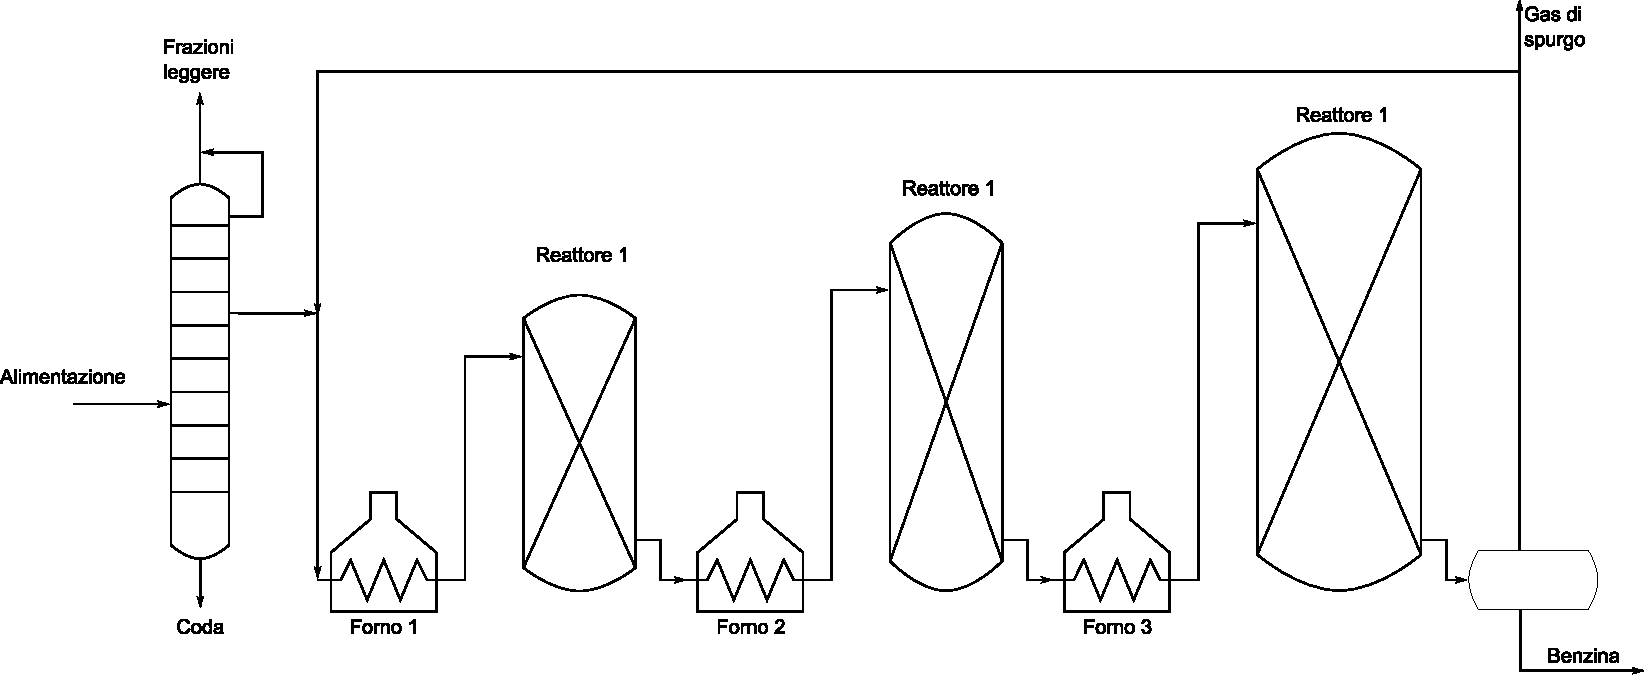
\includegraphics[width=0.85\textwidth]{image/ReformingPlantStaticBed}
		}
		\subfigure[Con reattori a letto fluidizzato]{
			\label{fig:Ref:Plant:FluidBed}
			
\includegraphics[width=0.85\textwidth]{image/ReformingPlantFluidBed}
		}
	\caption{Tipologie di impianti utilizzati per il cracking catalitico}
	\label{fig:Ref:Plant}
\end{figure}

\subsubsection{I reattori}
I reattori utilizzati sono reattori adiabatici di dimensioni crescenti; la dimensione dei reattori sono in funzione delle temperature raggiunte, infatti nel primo reattore si ha una pi� drastica riduzione della temperatura (il catalizzatore � attivo solo al di sopra di una certa temperatura critica), e quindi il tempo di contatto viene ridotto; la necessit� di avere dimensioni maggiori nei reattori successivi sono date anche dal fatto che le reazioni di deidrogenazioni (le pi� veloci ed endotermiche) avvengono nel primo reattore e per far progredire le reazioni pi� lente negli altri reattori sono necessari tempi di contatto maggiori.

Inizialmente costituiti da reattori a letto fisso a flusso assiale (\figurename~\ref{fig:Ref:Reattori:Assiale}), ci� per� portava a problematiche di rigenerazione del catalizzatore e difficile controllo delle temperature. Vennero di seguito sostituiti da reattori a flusso radiale (\figurename~\ref{fig:Ref:Reattori:Radiale}) che permettono un maggiore controllo termico e successivamente da reattori a letto fluido cosicch� il catalizzatore viene estratto e rigenerato in continuo.
\begin{figure}[htbp]
	\centering
		\subfigure[Flusso assiale]{
			\label{fig:Ref:Reattori:Assiale}
			
\includegraphics[width=0.25\textwidth]{image/ReattoreFlussoAssaile}
		}\quad\quad\quad\quad
		\subfigure[Flusso radiale]{
			\label{fig:Ref:Reattori:Radiale}
			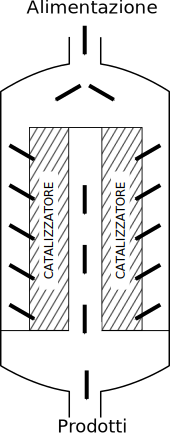
\includegraphics[width=0.25\textwidth]{image/ReattoreFlussoRadiale}
		}
	\caption{Tipologie di reattori utilizzati}
	\label{fig:Ref:Reattori}
\end{figure}

\subsubsection{La rigenerazione del catalizzatore}
Il catalizzatore utilizzato subisce disattivazione da parte di composti azotati e solforati, nonche dai metalli presenti che possono formare leghe con esso, infine il depositarsi di coke sulla superficie, per quanto limitato dall'elevata pressione parziale dell'idrogeno non pu� essere completamente evitato, quindi si ha riduzione della superficie attiva.

La rigenerazione del catalizzatore viene effettuata inizialmente procedendo ad una combustione con aria diluita da azoto per eliminare i residui carboniosi; si opera con una miscela povera di ossigeno, circa al 1-2\% e con temperature di circa $500^oC$.

La riattivazione della funzionalit� acida viene compiuta tramite un processo di ossiclorurazione che ha anche lo scopo di ridisperdere il platino presente all'interno; questa viene compiuta usando \ce{HCl} o una altra specie clorurante, vapore e ossigeno (circa al 10\%).

Nel caso in cui la funzionalit� di idrogenasi sia troppo elevata si pu� ricorrere ad un processo chiamato di \textit{tremperating} in cui si tratta il catalizzatore con una miscela di gas contenenti \ce{H_2S} ad una concentrazione di circa 100ppm.

Il catalizzatore di cracking catalitico pu� cos� essere rigenerato parecchie volte ed ha una vita utile di alcuni anni. Una volta sostituito il catalizzatore si procede ad un recupero di metalli preziosi presenti in esso (principalmente \ce{Pt} ma recentemente anche \ce{Re}).